% ------------------------------------------------------------------------
% ------------------------------------------------------------------------
% Monografia 2017
% Trabalho de Conclusão de Curso
% Baseia-se no documento modelo de TCC do abntex2
% Para saber mais, acesse https://github.com/abntex/abntex2
% ------------------------------------------------------------------------
% ------------------------------------------------------------------------

\documentclass[
		% -- opções da classe memoir --
		12pt,				% tamanho da fonte
		openright,			% capítulos começam em pág ímpar (insere página vazia caso preciso)
		oneside,			% para impressão em verso e anverso. Oposto a oneside
		a4paper,			% tamanho do papel.
		% -- opções da classe abntex2 --
		chapter=TITLE,		% títulos de capítulos convertidos em letras maiúsculas
		%section=TITLE,		% títulos de seções convertidos em letras maiúsculas
		%subsection=TITLE,	% títulos de subseções convertidos em letras maiúsculas
		%subsubsection=TITLE,% títulos de subsubseções convertidos em letras maiúsculas
		% -- opções do pacote babel --
		english,			% idioma adicional para hifenização
		brazil				% o último idioma é o principal do documento
	]{abntex2}


% ----------------------------------------------------------
% Pacotes básicos
% ----------------------------------------------------------
%\usepackage{helvet}
\usepackage[scaled]{helvet}
\renewcommand*\familydefault{\sfdefault} 	% Only if the base font of the document is to be sans serif
										% Foi necessário para acertar o documento, continha diversos erros
\usepackage[T1]{fontenc}		% Selecao de codigos de fonte.
\usepackage[utf8]{inputenc}	% Codificacao do documento (conversão automática dos acentos)
\usepackage{lastpage}		% Usado pela Ficha catalográfica
\usepackage{indentfirst}		% Indenta o primeiro parágrafo de cada seção.
\usepackage{color}			% Controle das cores
\usepackage{graphicx}		% Inclusão de gráficos
\usepackage{microtype} 		% para melhorias de justificação
% ----------------------------------------------------------


% ----------------------------------------------------------
% Pacotes adicionais, usados apenas no âmbito do Modelo Canônico do abnteX2
%% ----------------------------------------------------------
\usepackage{lipsum}				% para geração de dummy text
\usepackage{customizacoes} 		% customizações feitas pelo autor
% ----------------------------------------------------------
\usepackage{pdfpages}

% ----------------------------------------------------------
% Pacotes de citações
% ----------------------------------------------------------
\usepackage[alf]{abntex2cite}				% Citações padrão ABNT

% ----------------------------------------------------------
% CONFIGURAÇÕES DE PACOTES
% ----------------------------------------------------------

% ----------------------------------------------------------
% Configurações do pacote backref
% ----------------------------------------------------------
\definecolor{thered}{rgb}{0.65,0.04,0.07}
\definecolor{thegreen}{rgb}{0.06,0.44,0.08}
\definecolor{thegrey}{gray}{0.5}
\definecolor{theshade}{rgb}{1,1,0.97}
\definecolor{theframe}{gray}{0.6}
% ----------------------------------------------------------



% ----------------------------------------------------------
% Informações de dados para CAPA e FOLHA DE ROSTO
% ----------------------------------------------------------

\titulo{Desenvolvimento de um \emph{Framework} de linguagem interpretada para
processamento distribuído}
\autor{Vinicius Figueiredo Rodrigues}
\local{Bauru}
\data{2017}
\orientador{Profa. Dra. Roberta Spolon}

\instituicao{%
  Universidade Estadual Paulista "Júlio de Mesquita Filho"
  \par
  Faculdade de Ciências - Campus Bauru
  \par
  Departamento de Computação
}
\tipotrabalho{Monografia (Trabalho de Conclusão de Curso)}
% O preambulo deve conter o tipo do trabalho, o objetivo,
% o nome da instituição e a área de concentração
% foi necessário utilizar \~{a} e etc para os acentos por problemas na geração do PDF
\preambulo{Trabalho de Conclus\~{a}o do Curso de Bacharelado em Sistemas de Informação apresentado ao Departamento de Computa\c{c}\~{a}o da Faculdade de Ci\^{e}ncias da Universidade Estadual Paulista ``J\'{ú}lio de Mesquita Filho'' – UNESP, C\^{a}mpus de Bauru.}

% ----------------------------------------------------------


% ----------------------------------------------------------
% Configurações de aparência do PDF final
% ----------------------------------------------------------

% alterando o aspecto da cor azul
\definecolor{blue}{RGB}{0,0,0}

% informações do PDF
\makeatletter
\hypersetup{
     	%pagebackref=true,
		pdftitle={\@title},
		pdfauthor={\@author},
    	pdfsubject={\imprimirpreambulo},
	    pdfcreator={LaTeX with abnTeX2},
		pdfkeywords={big data}{sistemas distribuídos}{node.js}{abntex2}{trabalho acadêmico},
		colorlinks=true,       		% false: boxed links; true: colored links
    	linkcolor=blue,          	% color of internal links
    	citecolor=blue,        		% color of links to bibliography
    	filecolor=magenta,      		% color of file links
		urlcolor=blue,
		bookmarksdepth=4
}
\makeatother
% ----------------------------------------------------------


% ----------------------------------------------------------
% Espaçamentos entre linhas e parágrafos
% ----------------------------------------------------------

% O tamanho do parágrafo é dado por:
\setlength{\parindent}{1.3cm}

% Controle do espaçamento entre um parágrafo e outro:
\setlength{\parskip}{0.2cm}  % tente também \onelineskip

% ----------------------------------------------------------
% compila o indice
% ----------------------------------------------------------
\makeindex
% ----------------------------------------------------------


% ----------------------------------------------------------
% Configurações de projeto
% ----------------------------------------------------------
\newif\iffinal
\finaltrue % define se é um arquivo final, se for não for retira umas partes.

\newif\ifrelatorio
\relatoriofalse % define se é um arquivo final, se for não for retira umas partes.

\newif\ifabstract
\abstractfalse % define se mostra o abstract em inglês ou não.

\newif\ifresumo
\resumotrue % define se mostra o resumo ou não.

\newif\ifficha
\fichafalse % define se mostra a ficha catalográfica ou não
% ----------------------------------------------------------


% ----------------------------------------------------------
% Início do documento
% ----------------------------------------------------------
\begin{document}

% Seleciona o idioma do documento (conforme pacotes do babel)
%\selectlanguage{english}
\selectlanguage{brazil}

% Retira espaço extra obsoleto entre as frases.
\frenchspacing

% ----------------------------------------------------------
% ELEMENTOS PRÉ-TEXTUAIS
% ----------------------------------------------------------
\pretextual


% ----------------------------------------------------------
% Capa
% ----------------------------------------------------------
\imprimircapa
% ----------------------------------------------------------


% ----------------------------------------------------------
% Folha de rosto
% (o * indica que haverá a ficha bibliográfica)
% ----------------------------------------------------------
\imprimirfolhaderosto
% ----------------------------------------------------------


% ----------------------------------------------------------
% Inserir a ficha catalográfica
% ----------------------------------------------------------

% Isto é um exemplo de Ficha Catalográfica, ou "Dados internacionais de
% catalogação-na-publicação''. Você pode utilizar este modelo como referência.
% Porém, provavelmente a biblioteca da sua universidade lhe fornecerá um PDF
% com a ficha catalográfica definitiva após a defesa do trabalho. Quando estiver
% com o documento, salve-o como PDF no diretório do seu projeto e substitua todo
% o conteúdo de implementação deste arquivo pelo comando abaixo:
%
% \begin{fichacatalografica}
%     \includepdf{fig_ficha_catalografica.pdf}
% \end{fichacatalografica}

%\begin{fichacatalografica}
%	\sffamily
%	\vspace*{\fill}					% Posição vertical
%	\begin{center}					% Minipage Centralizado
%		\fbox{\begin{minipage}[c][8cm]{13.5cm}		% Largura
%				\small
%				\imprimirautor
%				%Sobrenome, Nome do autor
%
%				\hspace{0.5cm} \imprimirtitulo / \imprimirautor. --
%				\imprimirlocal, \imprimirdata-
%
%				\hspace{0.5cm} \pageref{LastPage} p. : il. (algumas color.) ; 30 cm.\\
%
%				\hspace{0.5cm} \imprimirorientadorRotulo~\imprimirorientador\\
%
%				\hspace{0.5cm}
%				\parbox[t]{\textwidth}{\imprimirtipotrabalho~--~\\ \imprimirinstituicao,
%					\imprimirdata.}\\
%
%				\hspace{0.5cm}
%				1. Balanceamento de Cargas.
%				2. Redes Neurais Artificiais.
%				3. Computação em Nuvem.
%				I. \imprimirorientador.
%				II. Universidade Estadual Paulista "Júlio de Mesquita Filho".
%				III. Faculdade de Ciências.
%				IV. \imprimirtitulo
%			\end{minipage}}
%		\end{center}
%	\end{fichacatalografica}

%\begin{fichacatalografica}
%	\ttfamily
%	\vspace*{\fill}					% Posição vertical
%	\hspace{1.5cm}
%	\begin{centering}	% Minipage Centralizado
%		\fbox{\begin{minipage}[c][7.5cm]{12.5cm}		% Largura
%				\footnotesize
%				\vspace{0.3cm}
%				\hspace{2.0cm} Setoue, Karoline Kimiko Figueiredo.
%				%Sobrenome, Nome do autor
%
%				\hspace{2.0cm} \parbox[t]{\textwidth}{\hspace{0.5cm} Aplicação de redes neurais artificiais no balanceamento de carga em serviços de nuvem / \imprimirautor, \imprimirdata} \\
%
%				\hspace{2.0cm} \parbox[t]{\textwidth}{\hspace{0.5cm} \pageref{LastPage} f. : il.} \\
%
%				\hspace{2.0cm} \parbox[t]{\textwidth}{\hspace{0.5cm} \imprimirorientador} \\
%
%				\hspace{2.0cm} \parbox[t]{\textwidth}{\hspace{0.5cm} Monografia (Graduação)~--~Universidade Estadual \\ Paulista. Faculdade de Ciências, Bauru, 2017 \\}
%				\\
%
%
%				\hspace{2.0cm} \parbox[t]{\textwidth}{\hspace{0.5cm} 1. Balanceamento de carga. 2. Redes neurais artificiais. \\ 3. Computação em nuvem. I. Universidade \\ Estadual Paulista. Faculdade de Ciências. II. Título.}
%			\end{minipage}}
%		\end{centering}
%\end{fichacatalografica}

 %\begin{fichacatalografica}
    % \includepdf{ficha.pdf}
 %\end{fichacatalografica}
% ----------------------------------------------------------


% ----------------------------------------------------------
% Inserir errata
% ----------------------------------------------------------
%\begin{errata}
%Elemento opcional da \citeonline[4.2.1.2]{NBR14724:2011}. Exemplo:

%\vspace{\onelineskip}

%FERRIGNO, C. R. A. \textbf{Tratamento de neoplasias ósseas apendiculares com
%reimplantação de enxerto ósseo autólogo autoclavado associado ao plasma
%rico em plaquetas}: estudo crítico na cirurgia de preservação de membro em
%cães. 2011. 128 f. Tese (Livre-Docência) - Faculdade de Medicina Veterinária e
%Zootecnia, Universidade de São Paulo, São Paulo, 2011.

%\begin{table}[htb]
%\center
%\footnotesize
%\begin{tabular}{|p{1.4cm}|p{1cm}|p{3cm}|p{3cm}|}
%  \hline
%   \textbf{Folha} & \textbf{Linha}  & \textbf{Onde se lê}  & \textbf{Leia-se}  \\
%    \hline
%    1 & 10 & auto-conclavo & autoconclavo\\
%   \hline
%\end{tabular}
%\end{table}

%\end{errata}
% ----------------------------------------------------------


% ----------------------------------------------------------
% Inserir folha de aprovação
% ----------------------------------------------------------

% Isto é um exemplo de Folha de aprovação, elemento obrigatório da NBR
% 14724/2011 (seção 4.2.1.3). Você pode utilizar este modelo até a aprovação
% do trabalho. Após isso, substitua todo o conteúdo deste arquivo por uma
% imagem da página assinada pela banca com o comando abaixo:
%
% \includepdf{folhadeaprovacao_final.pdf}
%
%\begin{folhadeaprovacao}

	%\begin{center}
		%{\ABNTEXchapterfont\large\imprimirautor}

		%\vspace*{\fill}\vspace*{\fill}
		%\begin{center}
			%\ABNTEXchapterfont\bfseries\Large\imprimirtitulo
		%\end{center}
		%\vspace*{\fill}

		%\hspace{.45\textwidth}
		%\begin{minipage}{.5\textwidth}
			%\imprimirpreambulo
		%\end{minipage}%
		%\vspace*{\fill}
	%%\end{center}

	%\center Banca Examinadora
	%\begin{center}
		%\vspace*{0.5cm}
		%\textbf{\imprimirorientador} \\ Orientador \\ Universidade Estadual Paulista "Júlio de Mesquita Filho" \\ Departamento de computação\\ Faculdade de Ciências \\
	%\end{center}
	%\begin{center}
		%\vspace*{0.5cm}
		%\textbf{Profa. Dra. Simone das Graças Domingues Prado} \\ Universidade Estadual Paulista "Júlio de Mesquita Filho" \\ Departamento de computação\\ Faculdade de Ciências \\
	%\end{center}
	%\begin{center}
		%\vspace*{0.5cm}
		%\textbf{Profa. Dra. Roberta Spolon} \\ Universidade Estadual Paulista "Júlio de Mesquita Filho" \\ Departamento de computação\\ Faculdade de Ciências \\
	%\end{center}
	%\assinatura{\textbf{Professor} \\ Convidado 3}
	%\assinatura{\textbf{Professor} \\ Convidado 4}

	%\begin{center}
		%\vspace*{0.5cm}
		%\par
		%{Bauru, 07 de Fevereiro de 2017.}
		%\vspace*{1cm}
	%\end{center}

%\end{folhadeaprovacao}
% ----------------------------------------------------------


% ----------------------------------------------------------
% Dedicatória
% ----------------------------------------------------------
%\ifrelatorio
	%\begin{dedicatoria}
		%\vspace*{\fill}
		%\centering
		%\noindent
		%\textit{ Este trabalho é dedicado às crianças adultas que,\\
		%		quando pequenas, sonharam em se tornar cientistas.}
		%\vspace*{\fill}
	%\end{dedicatoria}
%\fi
% ----------------------------------------------------------


% ----------------------------------------------------------
% Agradecimentos
% ----------------------------------------------------------
%\iffinal
	%\begin{agradecimentos}

	%\end{agradecimentos}
%\fi
% ----------------------------------------------------------


% ----------------------------------------------------------
% Epígrafe
% ----------------------------------------------------------
%\iffinal
	%\begin{epigrafe}
		%\vspace*{\fill}
		%	\begin{flushright}


		%\textit{"Mundo mundo vasto mundo..."\\
		%	(Carlos Drummond de Andrade)}
		%%\textit{""\\
		%		}
		%\end{flushright}
	%\end{epigrafe}
%\fi
% ----------------------------------------------------------


% ----------------------------------------------------------
% RESUMOS
% ----------------------------------------------------------
\ifresumo
	% resumo em português
	\setlength{\absparsep}{18pt} % ajusta o espaçamento dos parágrafos do resumo
	\begin{resumo}
			A partir da análise de ferramentas de processamento de \emph{Big Data} e
			\emph{Sistemas Distribuídos}, este projeto tem o intuito de criar um
			sistema de processamento paralelo em rede, com linguagem interpretada.

			O projeto consiste em um \emph{Framework} para possibilitar a distribuição das
			tarefas e uma aplicação que receberá e executará as tarefas distribuídas,
			conforme os detalhes passados pelo \emph{Framework}

		\textbf{Palavras-chave}: \emph{Big Data}. \emph{Sistemas Distribuídos}. Linguagem Interpretada. Processamento Paralelo.

	\end{resumo}

	% resumo em inglês
	% \begin{resumo}[Abstract]
	%  	\begin{otherlanguage*}{english}
  %   Based on the concepts of geomarketing, this work aims to develop a
  %   system that measures the traffic of people in certain zones using
  %   Wi-Fi network and mobile devices. In addition, it is intended to identify
  %   the profile of these individuals regarding the mobile device they use.
	%
	% 	\textbf{Keywords}: Geomarketing. People Traffic. Wi-Fi Networks. Mobile Devices.
	%
	% 	\end{otherlanguage*}
	%
	% \end{resumo}

\fi
% ----------------------------------------------------------


% ----------------------------------------------------------
% inserir lista de ilustrações
% ----------------------------------------------------------
% \iffinal
% 	\pdfbookmark[0]{\listfigurename}{lof}
% 	\listoffigures*
% 	\cleardoublepage
% \fi
% ----------------------------------------------------------


% ----------------------------------------------------------
% inserir lista de tabelas
% ----------------------------------------------------------
% \iffinal
% 	\pdfbookmark[0]{\listtablename}{lot}
% 	\listoftables*
% 	\cleardoublepage
% \fi
% ----------------------------------------------------------


% ----------------------------------------------------------
% inserir lista de abreviaturas e siglas
% ----------------------------------------------------------
% \iffinal
% 	\begin{siglas}
% 			\item[AP] Access Point - Ponto de Acesso
% 			\item[IoT] Internet of Things - Internet das Coisas
% 			\item[RFID] Radio-Frequency IDentification - Identificação por radiofrequência
% 			\item[TI] Tecnologia da Informação
% 			\item[Wi-Fi] Marca registrada da Wi-Fi Alliance. Rede local sem fios baseados no padrão IEEE 802.11
% 	\end{siglas}
% \fi
% ----------------------------------------------------------


% ----------------------------------------------------------
% inserir lista de símbolos
% ----------------------------------------------------------
%\iffinal
%	\begin{simbolos}
%			\item[$ \Gamma $] Letra grega Gama
%			\item[$ \Lambda $] Lambda
%			\item[$ \zeta $] Letra grega minúscula zeta
%			\item[$ \in $] Pertence
%	\end{simbolos}
%\fi
% ----------------------------------------------------------


% ----------------------------------------------------------
% inserir o sumario
% ----------------------------------------------------------
\pdfbookmark[0]{\contentsname}{toc}
\tableofcontents*
\cleardoublepage
% ----------------------------------------------------------



% ----------------------------------------------------------------------------------------------------------------------------------



% ----------------------------------------------------------------------------------------------------------------------------------
% ELEMENTOS TEXTUAIS
% ----------------------------------------------------------------------------------------------------------------------------------
\textual



\chapter{Introdução}
\label{introducao}

Em um ambiente em que a demanda computacional para processamento de dados e
execução de tarefas ultrapassa a capacidade computacional é necessário encontrar
maneiras diferentes de atender a demanda, como a utilização de sistemas
distribuídos, seguindo o conceito de divisão e conquista para atender as
necessidades do ambiente.

\section{Problema}
Com o crescimento de linguagens de interpretação é
importante que as mesmas tenham maneiras práticas de processar sua demanda
computacional, o que se torna uma tarefa difícil quando não se encontram pacotes
e bibliotecas de processamento distribuído dentre os grandes frameworks destas
linguagens.

\subsection{Solução proposta e motivação}
Tendo em mente o problema previamente descrito, o foco é o desenvolvimento
de um \emph{Framework} que permita o processamento distribuído para \emph{Node.js}, uma
plataforma de aplicações server-side com \emph{Javascript}, com recursos para
passar para outras máquinas tarefas e sua forma de execução.

\section{Objetivos}
\label{objetivos}

\subsection{Objetivos Gerais}
Este trabalho tem como objetivo desenvolver um \emph{Framework} para \emph{Node.js} que
permita o seu utilizador realizar o processamento distribuído de suas tarefas.

\subsection{Objetivos específicos}
\begin{itemize}
  \item Estudar as ferramentas que realizam processamento distribuído.
  \item Definir os tipos de tarefas a serem distribuídas.
  \item Definir interfaces para descrever as tarefas a serem distribuídas.
  \item Desenvolver um \emph{Framework} para distribuir as tarefas.
  \item Desenvolver uma aplicação para executar as tarefas distribuídas
  \item Testar a utilização da biblioteca em aplicações \emph{Javascript} de código aberto
  e de alto custo computacional
\end{itemize}

\section{Organização do trabalho}
O presente trabalho divide-se em seções, sendo esta a primeira (Introdução) e os demais na seguinte ordem:

\begin{itemize}
  \item \textbf{Fundamentação Teórica:} apresentação do embasamento teórico
  envolvidos no trabalho, e soluções semelhantes;
  \item \textbf{Metodologia:} ferramentas escolhidas para o desenvolvimento,
  e módulos do sistema;
  \item \textbf{Cronograma:} tarefas que serão realizadas dentro de seus
  respectivos prazos.
\end{itemize}
 % inclui o arquivo introducao.tex


\chapter{Fundamentação Teórica}
\label{fundamentacao-teorica}

% \subsection{Tipos de contadores}
% Não existe apenas um método para contar o número de pessoas. As principais
% diferenças entre os contadores estão em: área de cobertura, volume e tecnologia
% utilizada. Segundo \citeonline{wikipedia2017} e \citeonline{Ipsos} os principais métodos de
% contagem são:
%
% \begin{itemize}
%   \item \textbf{Feixes infravermelhos:} são colocados
% na entrada de lojas emitindo um feixe infravermelho entre os seus extremos,
% quando alguém interrompe o feixe, uma entrada é contada. A área de cobertura é
% pequena e o volume de pessoas que ele permite passando pela porta ao mesmo
% tempo é baixíssima;
%   \item \textbf{Câmeras termais:} o uso de sensores térmicos e
% processamento de imagens. Normalmente,
% são posicionados no teto para que a imagem capture a temperatura das pessoas
% e compare com a do ambiente. Este sistema permite alto volume de tráfego e instalação em entradas complexas.
%   \item \textbf{Vídeo:} Utilização de algoritmos complexos, inteligência artificial
%    e o processamento de imagens (2D e 3D). A área de cobertura
%   pode ser medida de acordo com o uso de câmeras e o volume permitido varia de acordo com os algoritmos.
%   \item \textbf{Wi-Fi:} utiliza o receptor Wi-Fi para pegar \emph{frames} únicos de gerenciamento Wi-Fi emitidos por dispositivos
%   dentro do alcance. Ideal para áreas onde o volume de pessoas é esparso ou incerto.
% \end{itemize}

% As escolha de um contador varia de acordo com a complexidade da entrada do lugar, períodos de captura do tráfego de pessoas,
% volume de pessoas por período, área de cobertura, precisão desejada, preço, entre outros \cite{trafsys} \cite{Axper2017}.
%
% \subsection{Área acadêmica}
% A principal técnica de contagem de pessoas pesquisada é por câmeras e processamento de imagens. Entretanto,
% as pesquisas diferenciam-se por técnicas de computação utilizadas. Alguns exemplos são:
%
% \begin{itemize}
%
%   \item \textbf{Robusto e leve:} com o objetivo de fornecer segurança para ambientes internos
%   o trabalho de \citeonline{Kim2002} preza por um sistema que seja robusto suficiente para garantir as metas, mas
%   não seja tão pesado do ponto de vista de algoritmos e demanda de hardware. O sistema reconhece o movimento de pessoas
%   ao longo de várias direções através de uma única câmera e um processador Pentium IV, assim ele estima e rastreia uma "caixa"  ao redor de cada indivíduo
%   para identificá-lo na imagem;
%
%   \item \textbf{Melhora no processamento de imagens e ruídos:} as pesquisas de \citeonline{Luo2016} e \citeonline{Hou2011} consideram
%   a queda de desempenho de sistemas de contagem em ambientes com multidões, oclusões (sombreamento/luminosidade
%   em cada quadro do vídeo) e informações de fundo complexas. O primeiro artigo propõe uma abordagem de cenas \emph{indoor}
%   que leva em conta multidões estacionárias (paradas) ou em movimento. O sistema detecta a multidão e separa
%   os ruídos. Depois, estima-se o número de pessoas através de "ombro-cabeça". Por fim, para reduzir as oclusões,
%   há um filtro que separa quadro por quadro do vídeo e faz um tratamento. Já o segundo, foca em subtrair o fundo, estima
%   o número de pessoas e utiliza técnicas para identificar as pessoas em imagens de baixa resolução;
%
%   \item \textbf{Múltiplos recursos:} os artigos de \citeonline{Venkatesh2015} e \citeonline{Ma2012} consideram múltiplos recursos para contar pessoas
%   em ambientes densos. O primeiro utiliza, principalmente, técnicas matemáticas e técnicas de filtros e imagens para estimar. Já o segundo, utiliza
%   múltiplas câmeras e vários níveis de textura para lidar com aparência humana e posições.
%
% \end{itemize}
%
%   As principais caraterísticas de sistemas de contagem que os artigos levantados focaram e presaram foram: movimentação das pessoas,
%   ambientes de multidão e processamento em tempo real.
%
% \subsection{Produtos na área empresarial}
% \label{produtos-empresas}
% Esta seção apresenta alguns contadores de algumas empresas. Na \autoref{density}, a empresa Density oferece a contagem a partir de um
% dispositivo localizado no topo da entrada que processa imagens 2D \cite{Density2017}. Já na \autoref{axper}, a empresa Axper além de oferecer
% o processamento de imagens 2D como a Density, oferece também um dispositivo que processa imagens 3D, cobrindo todo o ambiente \cite{Axper2017}.
%
% \begin{figure}[htb]
%   \caption{\label{density}Processamento de imagens 2D - Density People Counter}
%   \begin{center}
%     \includegraphics[width=0.40\textwidth]{img/density.png}
%   \end{center}
%   \legend{Fonte: \citeonline{Density2017}.}
% \end{figure}
 % inclui o arquivo fundamentacao.tex
%

\chapter{Materiais e Métodos}
\label{metodologia}
Este capítulo descreve o modo como a pesquisa, desenvolvimento e a documentação
do framework sugerido na \autoref{objetivos} será conduzida.

\section{Tecnologias utilizadas}
A escolha das tecnologias segue de acordo com a arquitetura do sistema.

\subsection{Javascript}
Para desenvolvimento do \emph{Framework} será utilizada a linguagem \emph{Javascript},
uma linguagem altamente difundida para desenvolvimento de páginas web.

Nos últimos anos a linguagem passou a ser usada também para desenvolvimento de
aplicações para servidor.


\subsection{Node.js}
Será utilizado o \emph{Node.js} como plataforma de execução do framework, ele
conta com recursos nativos do Sistema Operacional o que o torna extremamente
viável para o framework.


\subsection{Desenvolvimento}
Ao final do desenvolvimento, deveremos ter uma Aplicação, para realizar o
processamento das tarefas distribuídas, e um \emph{Framework} capaz de distribuir
tarefas em outras máquinas.


\subsubsection{Conexão}
O \emph{Framework} em sua inicialização receberá as informações, como
endere\c{c}o e detalhes de autenticação dos servidores que contém a aplicação que
processará as tarefas. A conexão, segundo o modelo de \citeonline{tanenbaum},
deve ser realizada utilizando o protocolo \emph{RTP}, um protocolo de
comunicação em tempo real baseado no protocolo \emph{UDP}, mas a implementação
será realizada utilizando o protocolo \emph{UDP}.


\subsubsection{Distribui\c{c}\~{a}o de tarefas}
O \emph{Framework} utilizará classes para:
\begin{itemize}
  \item Criação das tarefas;
  \item Configuração das tarefas;
  \item Distribuição das tarefas;
\end{itemize}

O fluxo da distribuição de tarefas seguirá o modelo da figura \ref{fig:dist-tarefas}.

Toda distribuição feita pela aplicação utilizando o framework deverá ser feita
por mensagens conforme o modelo a seguir:


\begin{lstlisting}[language=json, firstnumber=1]
{
  "id": Number,
  "start": Number,
  "size": Number,
  "dependencies": [String],
  "script": String
}
\end{lstlisting}

Onde \emph{``id''} será o código identificador utilizado internamente pela
aplicação, \emph{``start''} e \emph{``size''} delimitadores para o paralelismo
nos múltiplos computadores, \emph{``dependencies''} os \emph{pacotes}
necessários pelo processo e \emph{``script''} sendo o algoritmo que será
executado para cada conjunto de dados.

\begin{figure}[htb]
	\caption{\label{fig:dist-tarefas}Fluxo de tarefas distribuídas}
	\begin{center}
		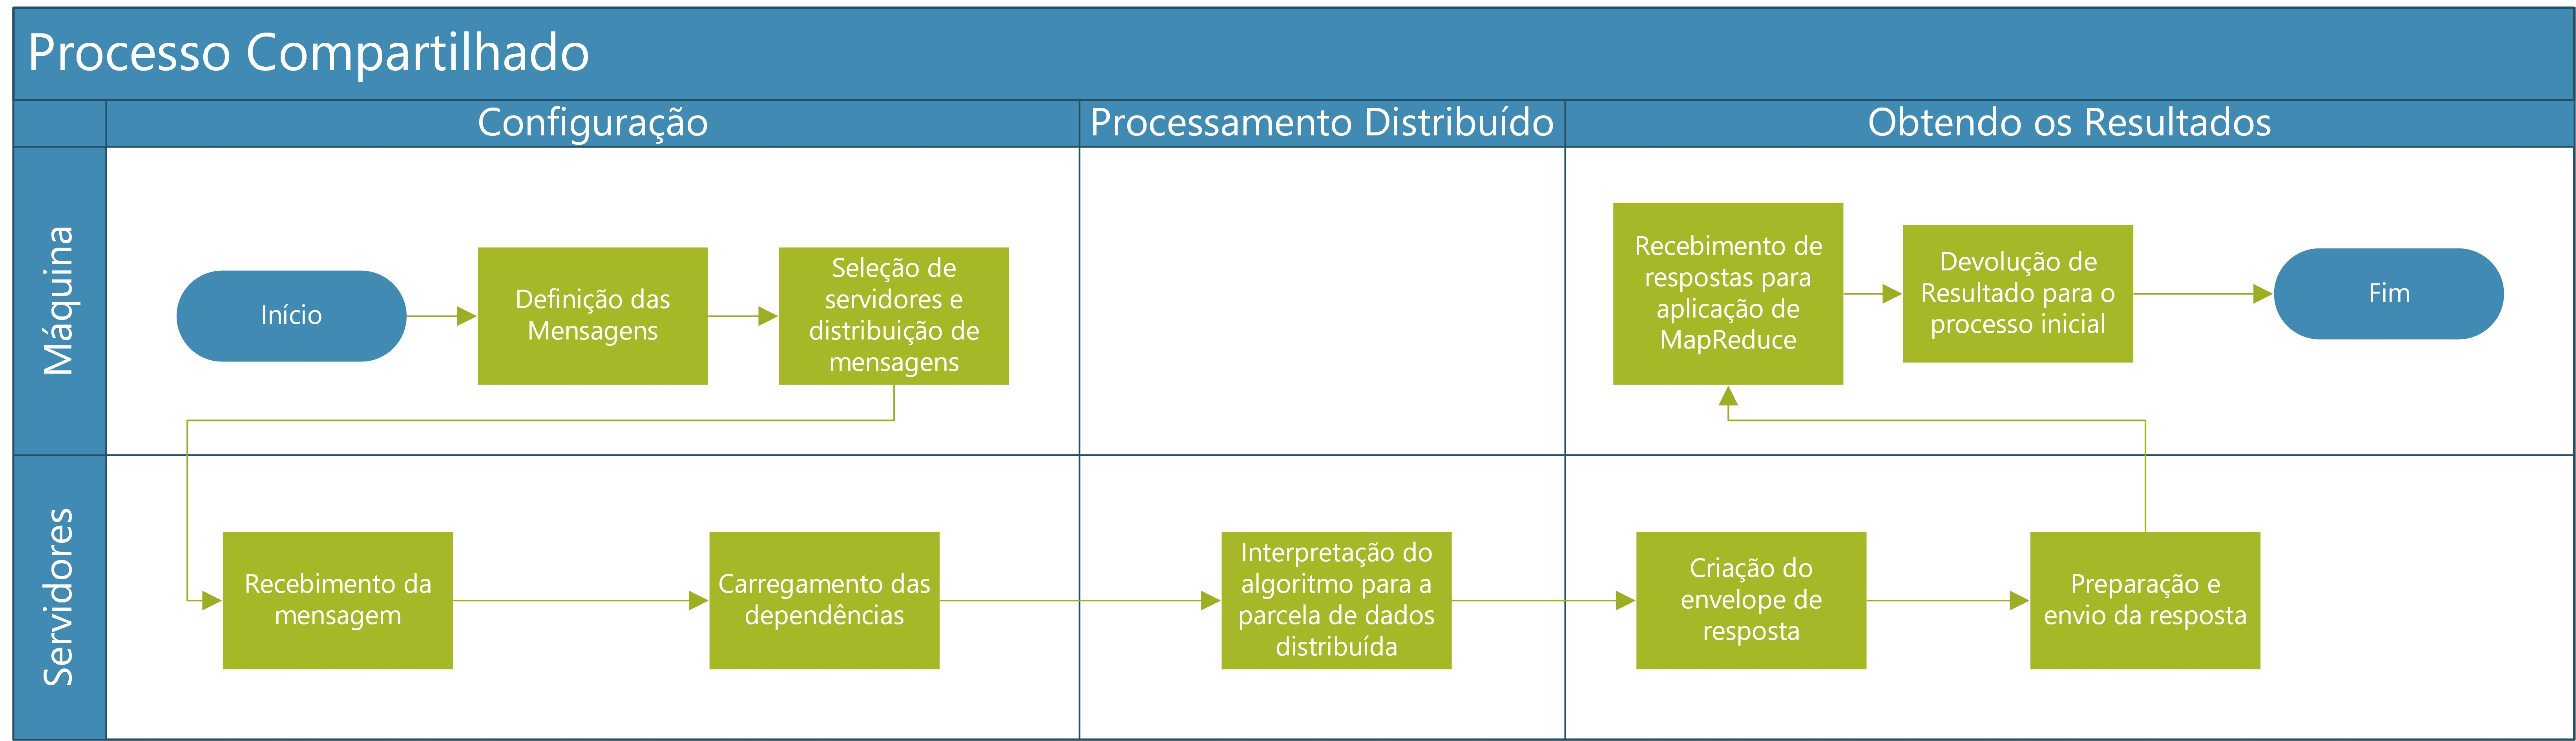
\includegraphics[width=1\textwidth]{img/processamento-distribuido.jpg}
	\end{center}
	\legend{Fonte: Elaborada pelo autor.}
\end{figure}

O processo de criação de uma chamada de procedimento remoto foi desenvolvido
tendo como base o modelo composto pelas etapas descritas por \citeonline{tanenbaum} na
figura \ref{fig:criacao-chamada}.

\begin{figure}[htb]
	\caption{\label{fig:criacao-chamada}Etapas na criação de uma chamada de procedimento remoto}
	\begin{center}
		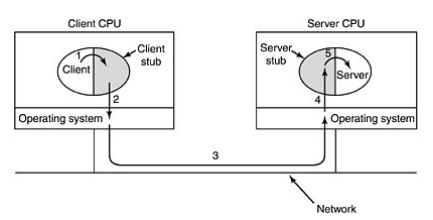
\includegraphics[width=1\textwidth]{img/criacao-chamada.jpg}
	\end{center}
	\legend{Fonte: Tanenbaum (2013).}
\end{figure}

A injeção de dependências será realizada internamente pelo servidor no processo
de carregamento de dependências seguindo o modelo da
figura \ref{fig:injecao-dependencias}.

\begin{figure}[htb]
	\caption{\label{fig:injecao-dependencias}Modelo de injeção de dependências}
	\begin{center}
		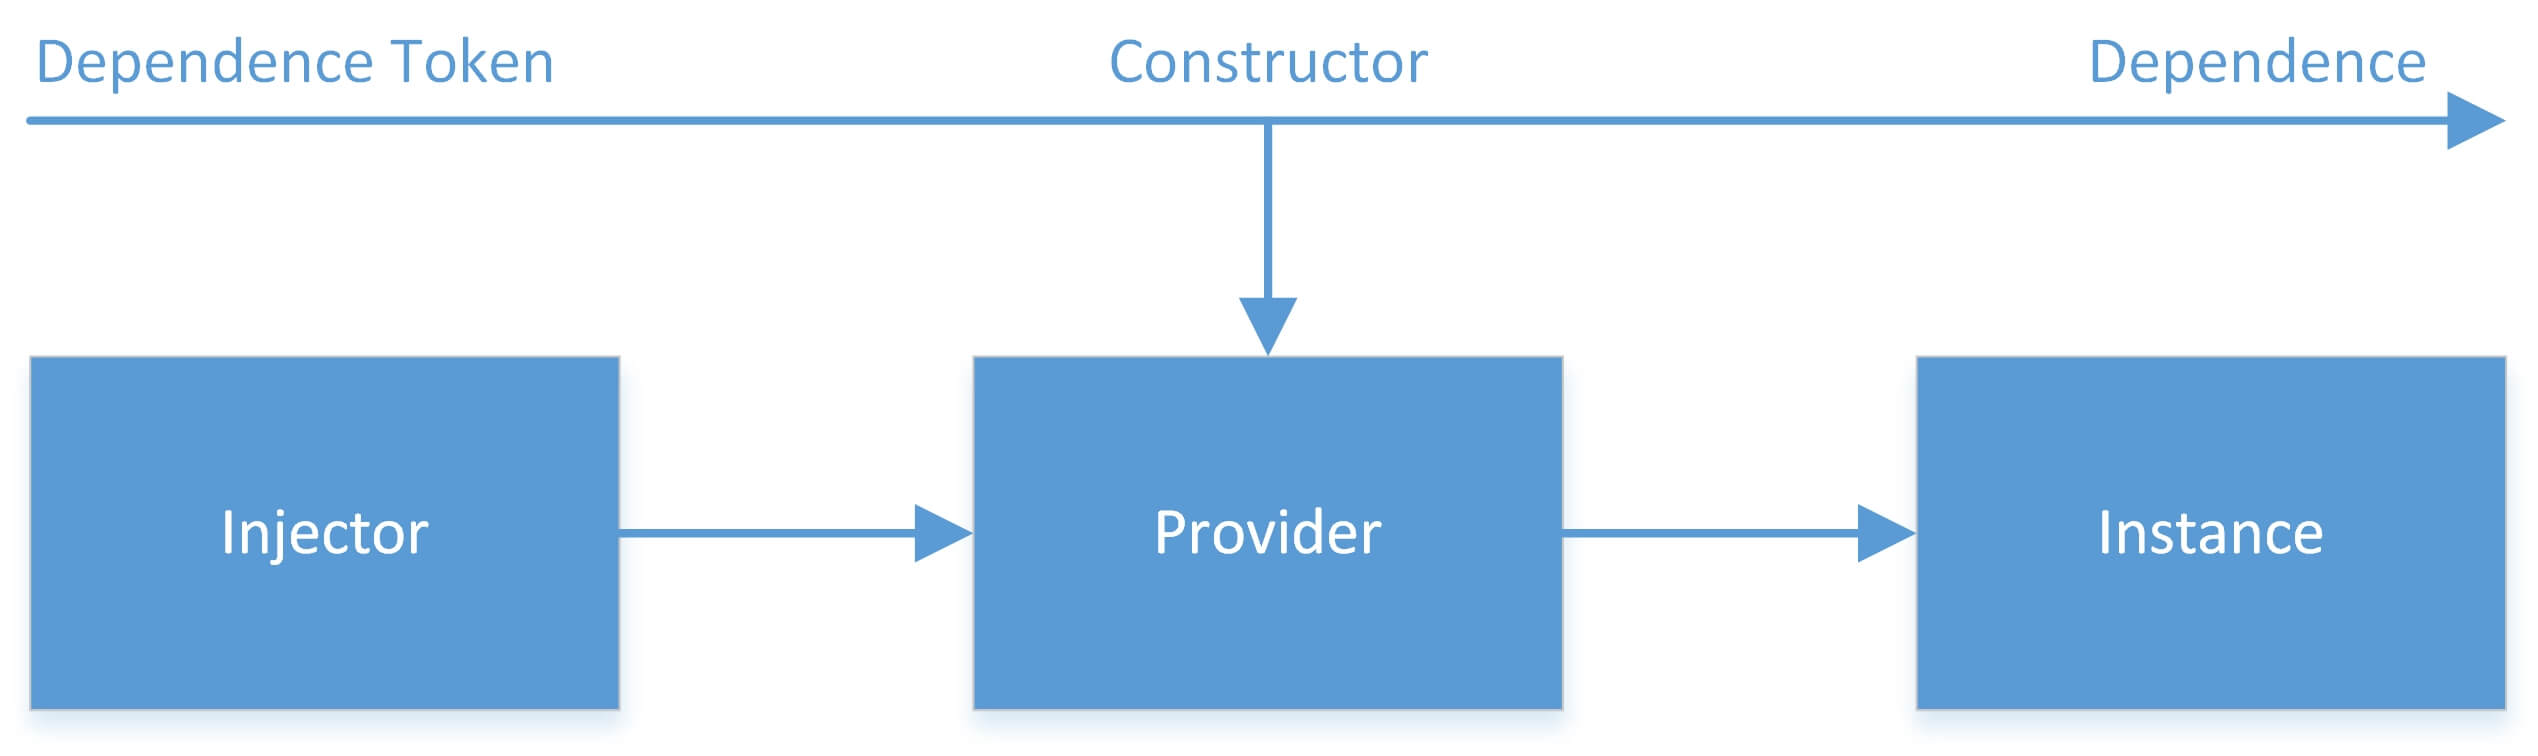
\includegraphics[width=1\textwidth]{img/injecao-dependencias.jpg}
	\end{center}
	\legend{Fonte: Elaborada pelo autor.}
\end{figure}

\pagebreak
\subsubsection{Aplicação para execução das tarefas}
A aplicação para distribuição também será feita utilizando \emph{Javascript} e
\emph{Node.js}. Ela interpretará a tarefas recebida e responderá para o
\emph{Framework} se ela foi executada corretamente ou não. Em caso de
\emph{MapReduce} também responderá com os dados processados.

\section{Padrões de Projeto}
O sistema utiliza os seguintes padrões de projeto baseados nos padrões de projeto da gangue
dos quatro definido no livro ``Design Patterns''.

\begin{itemize}
  \item \textbf{Command:} Modelo utilizado para padronização da execução interna
  de tarefas bem definidas, como inicialização e interrupção de processos;
  \item \textbf{Observer:} Modelo utilizado para aguardar mudanças na rede, como
  pedidos de execução de algoritmos, implementado no sistema em conjunto com o
  modelo de Command;
  \item \textbf{Factory:} Modelo utilizado para definir um padrão ao gerar
  objetos com bases em comum. Como no caso a criação e injeção de dependências.
\end{itemize}


Devido a utilização de uma linguagem interpretada, com poucos recursos de uma
linguagem orientada a objetos, se torna inviável a utilização de herança e fluxo
de informação à risca dos mesmos.

\section{Documentação}
Além da aplicação será necessário uma documentação bem descrita do código-fonte
e da arquitetura do sistema, abaixo serão descritas as ferramentas responsáveis
por esse requisito

\subsection{JSDoc}
\emph{JSDoc} é uma ferramenta utilizada para documentação de código-fonte em
\emph{Javascript}. A partir de comentários dentro do código-fonte é compilado um
conjunto de documentos responsáveis por descrever os \emph{módulos},
\emph{classes} e \emph{métodos} do código-fonte. Abaixo nas figuras
\ref{fig:jsdoc-js} e \ref{fig:jsdoc-html} exemplificam a entrada e saída de uma
documentação JSDoc.

\begin{figure}[htb]
	\caption{\label{fig:jsdoc-js}Exemplo de comentários no código-fonte para documentação}
	\begin{center}
		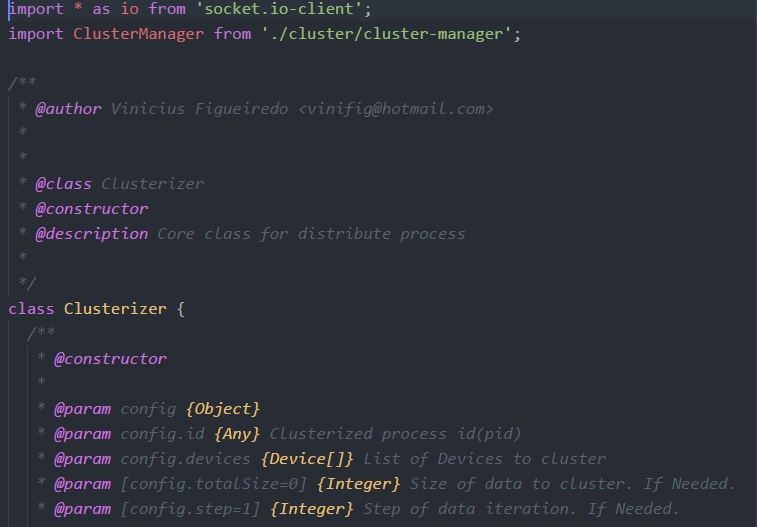
\includegraphics[width=1\textwidth]{img/jsdoc-js.jpg}
	\end{center}
	\legend{Fonte: Elaborada pelo autor.}
\end{figure}

\begin{figure}[htb]
	\caption{\label{fig:jsdoc-html}Exemplo de documento gerado pelo JSDoc}
	\begin{center}
		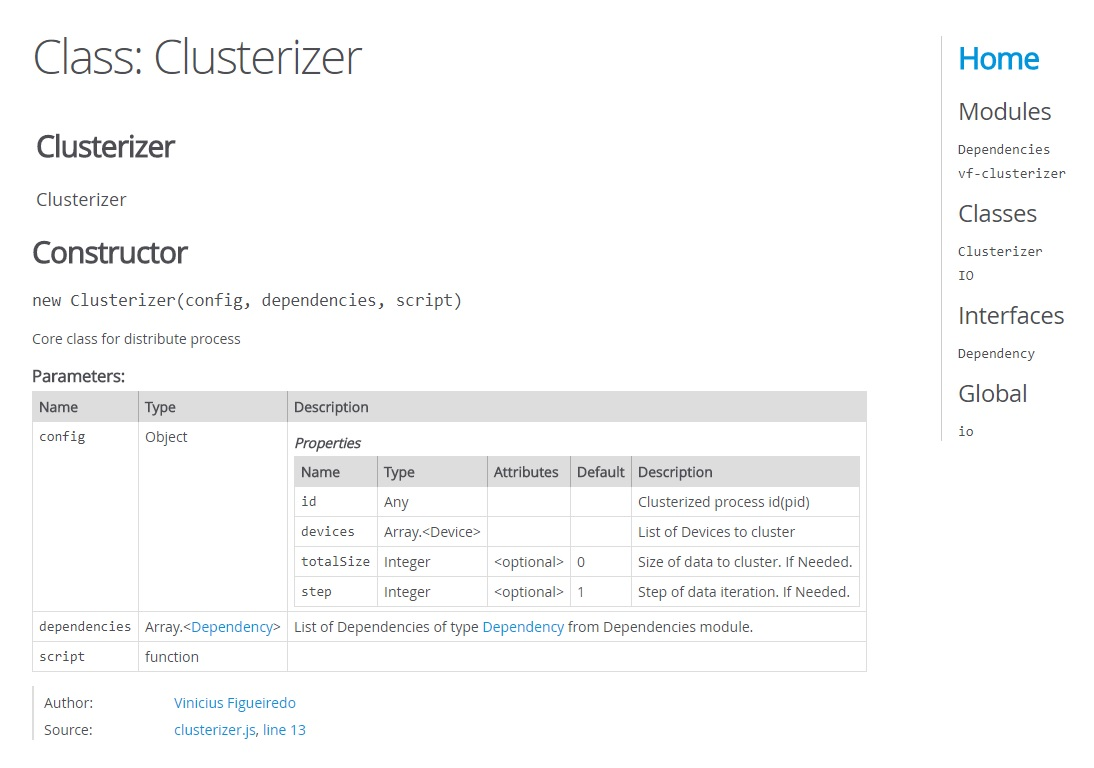
\includegraphics[width=1\textwidth]{img/jsdoc-html.jpg}
	\end{center}
	\legend{Fonte: Elaborada pelo autor.}
\end{figure}

\section{Protótipo}
Os requisitos funcionais definidos para o protótipo do sistema são:

\begin{itemize}
  \item Capacidade de comunicação entre as máquinas.
  \item Execução de comandos simples em outra máquina ou instância de software;
  \item Tratamento de erros de conexão.
  \item Documentação completa ou parcial do código-fonte existente.
\end{itemize}

Foram desenvolvidos um framework, responsável por auxiliar a comunicação da
aplicação \emph{client-side} com a aplicação \emph{server-side}. Abaixo na
figura \ref{fig:prototipo-resultado}, mostra um exemplo da execução da aplicação
definida na figura \ref{fig:prototipo-trecho-fonte} onde retorna
o horário em que foi executado cada iteração da tarefa distribuída.

\begin{figure}[htb]
	\caption{\label{fig:prototipo-trecho-fonte}Exemplo de código para
  distribuição de tarefas}
	\begin{center}
		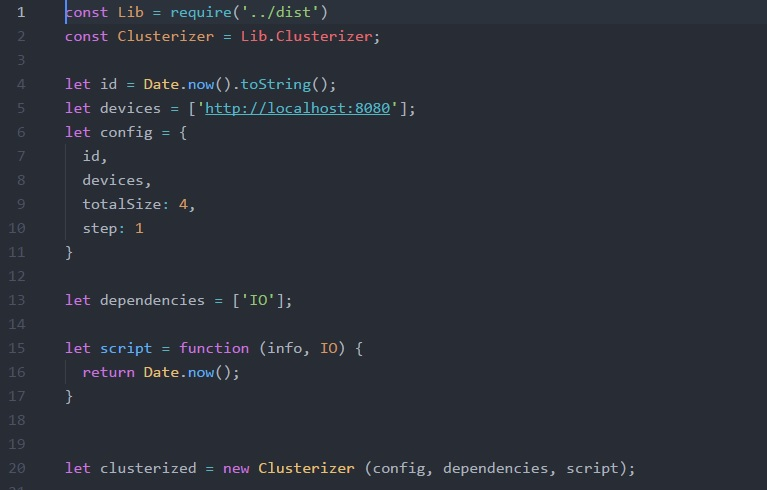
\includegraphics[width=1\textwidth]{img/prototipo-trecho-fonte.jpg}
	\end{center}
	\legend{Fonte: Elaborada pelo autor.}
\end{figure}

\begin{figure}[htb]
	\caption{\label{fig:prototipo-resultado}Exemplo de retorno de tarefa
  distribuída}
	\begin{center}
		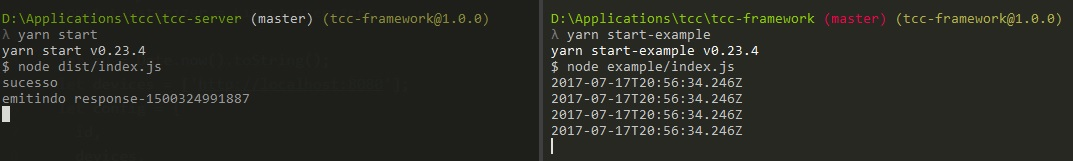
\includegraphics[width=1\textwidth]{img/prototipo-resultado.jpg}
	\end{center}
	\legend{Fonte: Elaborada pelo autor.}
\end{figure}
 % inclui o arquivo metodologia.tex
%
\chapter{Cronograma}
\label{cronograma}
O cronograma do trabalho está divido em duas tabelas: \autoref{tcc-1} sobre as entregas na disciplina de TCCI
e a \autoref{tcc-2} as entregas na disciplina de TCCII.

\begin{table}[h]
  \begin{center}
  	\caption{\label{tcc-1}Cronograma de atividades para o TCCI}
  	\begin{tabular}{c{4cm} c{2cm} c{2cm} c{2cm} c{2cm} c{2cm}}
      \hline
      Atividade & Abr & Mai & Jun & Jul & Ago \\
      \hline
      \hline
      Levantamento bibliográfico inicial & X & X & X \\
      \hline
      Definição das tecnologias & X & X & X \\
      \hline
      Definição dos tipos de tarefas &  & X \\
      \hline
      Definição da Interface de Comunica\c{c}\~{a}o &  & X \\
      \hline
      Documentação da arquitetura do sistema distribuído & & X & X \\
      \hline
      Desenvolvimento do \emph{Framework} & & & X & X & X \\
      \hline
      Desenvolvimento da Aplicação & & & X & X & X \\
      \hline
      Desenvolvimento de modelo de tarefa para teste & & & & X  \\
      \hline
      Teste e documentação do que foi desenvolvido & & & &  & X \\
      \hline
  	\end{tabular}
  	\legend{Fonte: Elaborado pelo autor.}
  \end{center}
\end{table}

\begin{table}[h]
  \begin{center}
  	\caption{\label{tcc-2}Cronograma de atividades para o TCCII}
  	\begin{tabular}{c{5cm} c{2cm} c{2cm} c{2cm} c{2cm} c{2cm}}
      \hline
      Atividade & Set & Out & Nov & Dez & Jan \\
      \hline
      \hline
      Desenvolvimento dos modelos de tarefa restantes & X & X & X & X & X\\
      \hline
      Pesquisa de aplicações para utilização do \emph{Framework}  &  & X & X \\
      \hline
      Testar o \emph{Framework} nas aplicações escolhidas & & X & X & X \\
      \hline
      Teste finais e validação & & & & & X \\
      \hline
  	\end{tabular}
  	\legend{Fonte: Elaborado pelo autor.}
  \end{center}
\end{table}

%
\chapter{Conclusão}
\label{conclusao}
O projeto consiste em desenvolver um \emph{Framework} para processamento
distribuído em \emph{Linguagem Interpretada}, no caso \emph{Javascript}, analisando
ferramentas já existentes.

A maior dificuldade do projeto será a execução do algoritmo distribuído, uma vez
que será definido pelo utilizador do \emph{Framework} e então distribuído para
as máquinas do sistema.
 % inclui o arquivo conclusao.tex

% ----------------------------------------------------------
% ELEMENTOS PÓS-TEXTUAIS
% ----------------------------------------------------------

% ----------------------------------------------------------
% Referências bibliográficas
% ----------------------------------------------------------
\bibliography{referencias}
% ----------------------------------------------------------

\end{document}
